\documentclass{article} % For LaTeX2e
\usepackage{nips15submit_e,times}
\usepackage{hyperref}
\usepackage{url}
\usepackage{times}
\usepackage{url}
\usepackage{graphicx}
\usepackage{amsmath}
\usepackage{bbm}
\usepackage{hyperref}
\usepackage{scabby}
\usepackage{tikz}
%\documentstyle[nips14submit_09,times,art10]{article} % For LaTeX 2.09

\newcommand\pl[1]{\textcolor{red}{[PL: #1]}}

\providecommand{\byt}{\hat{\by}}
\providecommand{\bys}{{\by^*}}
\providecommand{\yt}{\hat{y}}
\providecommand{\ys}{{y^*}}
\providecommand{\Regret}{\operatorname{Regret}}
\providecommand{\p}{p_{\theta}}
\providecommand{\e}{\epsilon}


%\input std-macros.tex


\title{Fake it until you make it:\\Asynchronous Bayesian Active Classification\\with Crowds}

\author{%
Keenon Werling\\
Department of Computer Science\\
Stanford University\\
\texttt{keenon@cs.stanford.edu} \\
\And
Arun Chaganty\\
Department of Computer Science\\
Stanford University\\
\texttt{chaganty@cs.stanford.edu} \\
\And
Percy Liang\\
Department of Computer Science\\
Stanford University\\
\texttt{liang@cs.stanford.edu} \\
\And
Chris Manning\\
Department of Computer Science\\
Stanford University\\
\texttt{manning@cs.stanford.edu} \\
}

% The \author macro works with any number of authors. There are two commands
% used to separate the names and addresses of multiple authors: \And and \AND.
%
% Using \And between authors leaves it to \LaTeX{} to determine where to break
% the lines. Using \AND forces a linebreak at that point. So, if \LaTeX{}
% puts 3 of 4 authors names on the first line, and the last on the second
% line, try using \AND instead of \And before the third author name.

\newcommand{\fix}{\marginpar{FIX}}
\newcommand{\new}{\marginpar{NEW}}

%\nipsfinalcopy % Uncomment for camera-ready version

\begin{document}

\usetikzlibrary{positioning}

\maketitle

\pl{I'd prefer a shorter title;
  not sure 'Fake it until you make it' is the right metaphor anyway
  since 'faking it' here actually means doing a good job too;
  if you want something fun, something along 'training wheels' or 'cyborg'?
  Something about smoothly transitioning from humans to machines in an online manner?
  Actually, why not call it LENSE?
}

\pl{not sure we actually want to pivot around the word 'active classification' so much;
I think we're sufficiently different from it; not only are they typically
not querying humans, but there's not a sense that the learning algorithm
gets better and the knowledge gets transfered from humans to computers,
which is \emph{the key point}}

\begin{abstract}
What if we could deploy a high-accuracy, real-time classification system, without expensive up-front data labelling?
We describe an ``on-the-job'' classification system, where as queries arrive, we use real-time crowdsourcing to resolve uncertainty where needed and output our prediction when confident.
As the model improves over time, the reliance on crowdsourcing queries decreases. 
We cast our setting as a stochastic game based on Bayesian decision theory, which allows us to balance latency, cost, and accuracy objectives in a principled way.
Computing the optimal policy is intractable, so we develop an approximation based on Monte Carlo Tree Search.
We tested our approach across three tasks---named-entity recognition, sentiment classification,
and image classification.
On the named-entity recognition task, we obtained a 6-7 fold reduction in cost compared to human classification, which requires multiple human votes to achieve the same level of accuracy.
We also achieve a 17\% F1 improvement over taking a single human vote as the answer to each query, and a 28\% F1 improvement over an online learning classifier that cannot query humans.
%Learning with little or no data is an important but understudied problem.
%For most tasks, the current paradigm of first collecting a training dataset and then training a classifier requires a substantial amount of data to be labeled to train a very accurate classifier.
%We propose a  that redistributes the same human effort to achieve
%better results faster: 
%query humans in real time at test time to train a machine learning system {\em
%on the job}.
%%\ac{is it clear what we're doing?}
%%The system only queries humans when it is unsure of its output and learns to 
%Querying humans introduces cost and latency but can improve accuracy over our
%model's prediction.
%We explicitly manage these three key objectives by casting the problem as a
%Bayesian decision theoretic control problem
%and draw on techniques from the game-playing literature.
%The resulting live system provides high quality responses in real-time while
%starting {\em with no training data\/}: we maintain $> 90\%$ F1 consistently on
%a stream of test inputs on the three tasks studied at low cost and latency,
%despite noisy labels from crowd workers.
% outperform baselines?
\end{abstract}

% V1
% Recent work in crowd-powered products has demonstrated the potential of using ``crowd workers'' to power live, low latency systems that accomplish AI complete tasks. 
% These systems suffer from high scaling cost, and the unreliability of workers.
% We propose an \textit{active classification} approach to dramatically reduce the scaling cost and improve the accuracy of such systems.
% In order to also achieve low latency, we investigate \textit{asynchronous} active classification, where multiple requests can be simultaneously ``in-flight.''
% This leads to the twin challenges of how to behave optimally in the presence of asynchronous noisy oracle queries that have not yet returned, and when to return a classification that is ``good enough'' in such a setting.
% We first reduce the problem of optimal asynchronous active classification to a Partial Monitoring game, by making use of Bayesian decision theory.
% We show a bound on achievable regret in this setting, and demonstrate practical heuristics that approach this bound.
% We also show adaptations for traditional Active Learning algorithms to our setting.
% We show empirical demonstration of our proposed algorithms, which demonstrate dramatic improvement over the human-only, machine-only, and baseline human-machine hybrid alternatives in the cost-delay-accuracy tradeoff surface.

% V2?
% Recent work in real-time crowd-powered products has demonstrated the possibility of using human ``crowd workers'' to power live, low latency products that accomplish AI complete tasks. Human-only solutions remain expensive, and do not scale into production. We propose a \textit{active classification} approach to dramatically reduce the scaling cost of such systems, backed by a pool of unreliable crowd-workers. In order to achieve this, we investigate \textit{asynchronous active classification}, where multiple requests can be simultaneously ``in-flight.'' This paper analyzes the \textit{asynchronous requests problem} of how to behave optimally in the presence of asynchronous oracle queries that have not yet returned, and the \textit{optimal stopping problem} of when a classification is ``good enough'' in such a setting. Our solutions to these problems enable a system that shows dramatic improvement over the human-only, machine-only, and baseline human-machine hybrid alternatives in the cost-delay-accuracy tradeoff surface.
% With sufficient labeled data and research effort, supervised learning has been applied in performance critical domains.
% Yet, often logistical/financial constraints mean that data can only be collected and labeled in the presence of a working system, or that insufficient data can be collected to achieve performance requirements.

% V3
% We propose a crowd/machine learning hybrid approach to apply supervised learning in performance critical domains where ``cold start'' barriers exist: we allow our model to query the crowd in real-time {\em at test time}, and learn from the crowd responses online to improve performance and reduce costs on future inputs.
% %Querying humans in real time introduces latency, noise, and cost into the system, which must be minimized.
% Querying humans introduces latency, noise, and cost into the system, which must be minimized.
% We explicitly manage these three key objectives by casting the problem as a Bayesian decision theoretic control problem, and drawing on techniques from game-playing literature for real-time solutions.
% The resulting system provides high quality responses in real-time while starting {\em with no training data\/}: we have achieve $> 90\%$ F1 on the three tasks studied at a low cost, despite noisy crowd worker performance.
% % outperform baselines?


%\section{TODO}

\subsection{Arun}

\begin{itemize}
  \item I don't like that "money" and "time" are explicit variables in the loss function, mainly because it seems too concrete for abstract math. We can choose an specific loss function at a later time dependent on those parameters. I might yet come around to this notation.
\end{itemize}


\section{Introduction}

\begin{epigraph}
``It ain't what you don't know that gets you into trouble.\\
It's what you know for sure that just ain't so.'' \\
-- Mark Twain
\end{epigraph}

For the practitioner, supervised learning is largely a solved problem and software to efficiently train classifiers in a variety of domains is readily available.
Yet, adoption remains limited because the deployment of a learning system requires extremely accurate classifiers: mistakes cost business.
The typical solution to this problem is to use more labeled data, which recent crowdsourcing platforms such as Amazon Mechanical Turk or CrowdFlower have made relatively affordable to obtain\findcite{citefest!}.
However, this not only presupposes the ready availability of large amounts of unlabeled data, but also advocates a long, expensive data collection process for uncertain improvements in accuracy.
% This two-stage process fundamentally limits the accuracy we can obtain.
An alternate approach is to use cut out the middle man altogether and use the crowd to label all examples in real-time\cite{cheng2015flock}. 
While this allows us to ensure accurate responses, it becomes prohibitively expensive to scale to more data. 

Our approach interpolates between these two regimes: we query the crowd in real-time when our model is unsure and learn on the crowd responses to improve on future input.
This results in a system that provides users high quality responses in real-time while starting {\em with no training data}.
In this paper, we explicitly address three main challenges that arise in doing so: keeping costs low, guaranteeing low latency and maximizing accuracy.

Let us explore an example use-case for such a framework:
\begin{example*}[Extracting fields from online classifieds]
  \todo{arun: make sexy!}
  You wish to create an online classifieds for apartment listings. 
  Your USP is to automatically identify salient features like the number of bedrooms, housing features, the date of an open house, etc. to allow users to search for listings that match their requirements.
  A successful service will receive thousands of such postings every day, making manual classification impractical.

  Something about starting with zero training data.

  \todo{arun: maybe the rest of the description of the system is in relation to this example}
  Using the system described in this paper, you, the owner, need to specify a model to use - in this case, a linear chain conditional random field is relevant.
  The next challenge is getting data. 
  On each example we can get crowd workers to identify these features, an easy task for people.
  There is a variety of tasks that you can ask people - identifying dates might be easier than not. 
  Could ask people to identify what a particular word, say pool, is.
  Alternatively, you could ask people to identify the nearest landmark.

  This data incorporated into the system to provide a more accurate labeling in the future.
\end{example*}

% Cost and Low-latency
We focus on structured classification problems using conditional exponential families, a general model class that has been used to \todo{citefest}. In such a model, we are given an input, $\bx$, and must predict a number of labels $\by = y_1, \ldots y_n$.

We treat crowd workers as a resource that can provide noisy measurements of some subset of the labels.
Under time and budget constraints, we must optimize over which labels to query when. 
Often, several queries are required on a particular label because of annotator errors by the crowdworker, while at other times it is better to distribute queries across labels.
Similarly, observing a label from one worker lets us decide better which label to query next, but we might not have to time to wait for the response.

We propose an active classification approach using Bayesian decision theory that is able to make these complex behavioral decisions.
This quickly leads to an intractable optimization problem that grows exponentially in complexity with the number of label queries we might ask on a single example.
We propose a novel approximation based on Monte Carlo tree search that retains the behavior of the original Bayesian approach while being computationally tractable.

\todo{(arun): We should make the distinction with active learning much stronger since that's what everyone thinks we're doing. I've moved the related work section to the latter parts because I feel like it's easier to compare our work with existing work given our model.} 

Finally, in practice, labels from crowd workers are often inaccurate.
We use the measurements framework of Liang et.\ al\cite{liang09measurements} to incorporate noisy responses from crowdworkers in our model.
Having an accurate estimate of the error rates for crowd workers is essential to accurately predicting how many queries are required.
Prior work\findcite{unsupervised crowd labeling} uses inter-annotator agreement to predict per-user error rates in an unsupervised manner. 
The online nature of our task limits the number of responses we have on the same label.
Instead, we learn the error rates in an unsupervised fashion using online EM, which also allows us to incorporate unlabeled data.

% Experiments
We evaluate our system on four different tasks: named entity recognition, information extraction from user generated content, image classification and sentiment classification on tweets.
We show that by querying crowdworkers at classification time, we can significantly outperform a system trained on fully labeled data, for a fraction of the cost of the baseline of asking crowdworkers for labels for each example, as well as the system trained on fully labeled past data.
On X of the Y tasks, we produce a classifier comparable with the state of the art while obtaining a much smaller subset of the training labels noisily from the crowd. 
In fact, we are comparable with state of the art-ish with a handful of the training labels.
An open-source implementation of our system will be made available.

% Recent work has shown that it is possible to use real-time on-demand workers to power everything from AI-complete email clients~\cite{kokkalis2013emailvalet} to real-time activity surveillance and classification~\cite{lasecki2013real}.
% These purely crowd-based solutions are prohibitively expensive at scale.
% Powering the crowd-based email client \textit{EmailValet}~\cite{kokkalis2013emailvalet} for a single end user for a year costs over \$400.
% 
% These systems typically work by ``pooling'' on-demand workers from high latency job-posting platforms like Amazon Mechanical Turk or CrowdFlower on a website designed by the system architect~\cite{lasecki2011real}.
%  The ``pooling'' process can take several minutes, but once in place the workers can be queried at very low latencies by pushing requests to their web-browsers.
%  This pool of workers can demonstrate high rates of turnover, and unreliability amongst individual annotators.
% 
% Existing systems query this pool directly, allowing for annotator noise by incorporating consensus building systems like voting and chat.
% 
% 
% Active classification~\cite{greiner2002learning}, a close sibling of active learning, is a setting in which a classifier is allowed to query for more information, at some cost, before turning in classifications.
%  This active classifier is intended to reduce its need for costly, slow human labels over time by learning from past observations.
%  We propose to adapt the active classification framework to the pooled-worker setting to query this pool more cheaply, accurately, and quickly, without sacrificing the advantages live of crowd-powered interfaces.
% 
% Previous work in online active learning (which is closely related to what we're proposing) has focused on multi-class classification (\cite{chu2011unbiased},~\cite{agarwal2013selective},~\cite{cheng2013feedback},~\cite{vzliobaite2011active},~\cite{helmbold1997some}).
%  Multi-class classification is an insufficiently rich primitive to handle many of the tasks that crowd-workers are enabling in existing systems, like information extraction or object detection.
%  Instead, we will build our platform around arbitrary log-linear markov network classification, where we assume it is possible to query workers for opinions on individual nodes.
%  Thus each ``active classification'' in our proposed setting is instantiate with a markov network and involves using model priors trained on previously seen data to choose to query the worker-pool for opinions about nodes, and then returning a classification informed by those opinions.
% 
% 
% This setting poses several distinct challenges that have not been sufficiently addressed in previous literature.
%  We need to be sensitive to time delays, returning results at least as quickly as the pure-crowd baseline we intend to improve upon.
%  We also need to be sensitive to inaccurate oracles.
%  These two criteria, in the pooled-worker setting, means that we need an active classifier who is able to hide latencies of redundant queries by launching them \textit{asynchronously}.
%  This leads to the two challenges we will address in this paper, which can both be clustered under \textit{optimal asynchronous behavior}: we need to be able to handle the decision to ask for another query or turn in existing results in the presence of ``in-flight requests,'' which can fail due to worker turnover, where our loss term is sensitive to time delay.
%  We draw inspiration from work in Bayesian Active Learning to tackle these problems.




\section{Problem setup}
\label{sec:model}

\pldone{I'd start out with the overarching problem setting \emph{independent} of our approach.
  Since this is a novel setting, let's make it objective; you don't have to use Bayesian decision theory
  to solve it.
In particular, talk about the inputs, the outputs, the measurements, the online setting, latency, cost, etc.,
but no model, no algorithms.
}{see below}

Let us formalize our problem setting. %, using the disaster relief example from the introduction to make things concrete.
We receive a stream of inputs $\bx\oft1, \bx\oft2, \ldots, \bx\oft t$ with corresponding {\em unobserved\/} true labels $\by\oft1, \by\oft2, \ldots, \by\oft t$ that we would like to predict.
For each input, we are allowed to ask workers for partial observations on the labels at a specified cost per label.
Note that the responses we receive can be (and often are) inaccurate and the requests introduce latency.
After making some number of requests, our system must return a prediction, $\byt\oft{t}$.
Our goal is to maximize accuracy trading off cost and latency as specified by a given objective function.

More formally, suppose the output $\by\oft{t}$ has $n$ parts: $\by\oft{t} = y\oft{t}_1, \dots, y\oft{t}_n$.
Let $q\oft{t} \in \{1, \ldots, n\}$ be a request for the label $y\oft{t}_q$,
let $Q\oft{t} = (q\oft{t}_1, \dots, q\oft{t}_m)$ be a sequence of queries made on the $t$-th input and
let $\tau\oft{t}$ be the time taken to make the prediction $\byt\oft{t}$. 
We would like to minimize the cumulative misclassification loss, 
following objective:
\begin{align}
  \sL &= \sum_{t=1}^T \ell(\by\oft{t}, \byt\oft{t}) + C(Q\oft{t}, \tau\oft{t}), \label{eqn:objective}
\end{align}
where $\ell$ is a given loss function, e.g.\ the Hamming loss, and $C$ is a given cost function.
\ac{Concern: by using the cumulative loss, is there an expectation that we will ``model'' input and optimize for the future?}

We now describe our choice of models for prediction, human error and latencies and return to optimizing \equationref{objective} in \sectionref{async}.

% A general model family - conditional exponential models
% Incorporating feedback as "measurements" as per Percy
% Error model - defer investigation to a later section.
% Querying for an optimal measurement - defer asynchrony to a later section.
% Learning given feedback 

%\pl{Also, the measurement stuff gets kind of abstract quickly, so have good running examples
%and try to minimize notation; don't go for generality if you don't need it}

%Our goal, given an existing model, is to identify labels where we lack confidence, query crowd works for measurements if needed and incorporate the resultant responses back into our model.
\paragraph{Prediction model}
We consider the family of conditional exponential models, a popular class of models that include logistic regression and conditional random fields.
Let $\bx$ be a given input, then the labels $\by = y_1, \ldots, y_n \in \{1, \dots, L\}$ are generated by the following conditional distribution:
\begin{align*}
  \p(\by \given \bx) 
  &= \exp( \theta^\top \phi(\bx, \by) - A(\theta; \bx)),
\end{align*}
where $\theta$ are the model parameters,
$\phi(\bx, \by)$ are arbitrary features of the input and labels and 
$A(\theta; \bx)$ is the conditional log-normalizer.
We assume that the model has low treewidth (e.g.\ $\phi$ factorizes over the labels $\by$) or otherwise admits efficient marginal computation.

In our running example of identifying actionable items from Twitter messages, the model is a linear-chain conditional random field (\figureref{crf}). The input is the sequence of words in the tweet, the output is a label in the set $\{\textsc{none}, \textsc{food-source},  \textsc{food-request}, \dots\}$. Marginal inference can be efficiently computed using the Viterbi algorithm.

\pldone{need a concrete example of what $\tau_\sigma$ is; a small example with actual labels;
in general, not sure if you want to use measurements here
}{restricted measurements to be at the label level, also concrete example now}

\begin{figure}[t]
  \begin{centering}
  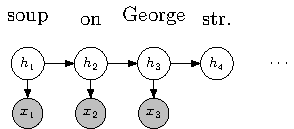
\includegraphics[width=0.5\textwidth]{figures/simple-crf.pdf}
  \end{centering}
  \caption{A conditional random field \todo{(arun): make a CRF and show what happens when measurements are added.}}
\label{fig:crf}
\end{figure}

%Conventionally, we are given a training dataset $\sD = \{\bx_i, \by_i\}$ and can learn $\theta$ by optimizing the convex log-likelihood objective $\sL(\theta) = \sum_{t=1}^T \log \p(\by\oft{t} \given \bx\oft{t})$.
%In our setting, however, we do not observe the gold labels $\by$. 
%Instead, we can ask the crowd to provide a ``measurement'' for some subset of the labels.
%Let $\Sigma = \{\sigma_i\}$ be the set of possible measurements we can ask the crowd for and 
%let $\by_\sigma \subseteq \by$ be the subset of labels queried.

\paragraph{Human error model}
We also model the responses, $z_q$, with an exponential measurement model:
\begin{align*}
  p(z_q \given x, y) 
  &\propto \exp \left( \omega^\top\psi(\bx, y_q, z_q) \right),
\end{align*}
where $\omega$ and $\psi$ are extra parameters and features for the human error model. 
%The choice of an exponential model allows us to simply include measurements as an additional factor.
\figureref{crf} shows the original graph with additional measurement nodes.
A simple human error model is to return the true label with probability $1-\epsilon$ and a random label otherwise.
In our running example, some classes, e.g.\ $\textsc{none}$, are more easily identified than others: in this setting human responses can be modeled to be sampled from a confusion matrix.

Finally, we model delay to be drawn from a Gamma distribution: $\tau_q \sim \Gamma$\footnote{We assume that the response delays are independent of the input and which label is being queried, though the model can easily be generalized to this setting.}.
The total time taken on a prediction, $\tau$, depends not only on how many requests are made, but also when they are scheduled.
We study the problem of how to best schedule multiple requests in \sectionref{async}.


%In the simplest case, assume the labeler returns the true label with a uniform probability of $1- \epsilon$, and guesses at random otherwise, $\theta'$ and $\phi'$ are:
%\begin{align*}
%  \theta' &= 
%      \begin{bmatrix}
%        1 - \e \\ \e
%      \end{bmatrix} &
%  \phi'(\tau_q, \by_q, \bx) &=
%    \begin{bmatrix}
%      \BI[\tau_q = y_q] \\
%      \BI[\tau_q \neq y_q]
%    \end{bmatrix}.
%\end{align*}
%Independently, we model the time each measurement takes, $D_q$.
%We revisit the problem of learning the error distribution of labelers in \sectionref{human-error}.

Next, we describe how we use our models to predict labels and learn from partial feedback.

\paragraph{Prediction}
Given parameters $\theta, \omega$ and measurement responses $z_1, \ldots, z_n$, we query for predictions using a maximum likelihood labeling:
$\byt \given \bx, z_1, \ldots z_m = \argmax_{\by} \p(\by \given \bx, z_1, \ldots z_n)$.

\paragraph{Learning from responses}

Recall that we do not have gold labels for our data, but only noisy measurements: we do not have supervised examples to learn from. 
As a simple heuristic, we use the output from our model as gold labels and update our parameters periodically.  
In future work, we plan to explore using (online) expectation-maximization to jointly learn parameters for our model and the human error model in an unsupervised fashion.

%\section{Theoretical Bounds on Active Classification Performance}
\label{sec:bounds}

We're interested in providing extreme limits of classifier performance under an unrealistic set of assumptions, as a way to gain intuition about the setting and the limitations of our approach.
It's trivially easy to see that it is possible to spend no money, and no time, during classifications. Simply return null on every request.
It's more interesting to evaluate if it's possible to return a perfect classification every time, and how much we have to give up in average cost to achieve perfection.
Let's assume that our temporal and financial budgets are infinite, we have an infinite number of humans on call, and we have an accurate model of the confusion matrix of humans $C$.
If all of these conditions are met, are there any guarantees we can make about our classifier?
Trivially, if our classifier always returns a uniform distribution over all possible output labels, and we query an infinite number of humans, it is possible to achieve arbitrary accuracy.
More interestingly, are there non-trivial bounds we can set on the cost-guarantee tradeoffs?

As an overview, our analysis will first define the value of valid priors on the data in terms of number of human queries required, under some simplifying assumptions about human error.
We will then focus on the challenge of not being able to absolutely trust model confidence estimates.
We define a rigorous way of conceptualizing ``trust'' in our confidence values, which requires defining the set of ``true confidence'' estimates allowable by the data for a given input.
Then we define bounds of expected classification performance given a choice for this ``trust,'' and demonstrate that more trust leads to higher error rates and lower costs.

\subsection{True Confidence Values}

First we must define the set of ``true confidence'' distributions $\Delta$.
Let data arrive in the form of $(\bx_i,\by_i)$ pairs, where $\by_i$ is the always observed set of variables we condition on, and $\bx_i$ is the true observed outcome.
Given a set $\Gamma$ of IID pairs, a norm $N$, and a feature mapping $f(\by) = \bz \in \sR^m$,
 let the ``$\epsilon$-neighborhood'' of $\by_t$ (notation $\Gamma(\epsilon, \by_t)$) be defined as all pairs in $\Gamma$ within the norm ball under $N$ of size $\epsilon$:
\[\Gamma(\epsilon, \by_t) = \{\bx_i \in \Gamma | ||f(\by_i) - f(\by_t)||_N \leq \epsilon\}\]
Every $\epsilon$-neighborhood, for $\epsilon \in \sR^+$, defines a natural frequentist estimate for $P(\bx_t | \by_t)$:
\[P(\bx_t | \by_t; \epsilon) \approx \sum \frac{\Gamma(\epsilon, \by_t)}{|\Gamma(\epsilon, \by_t)|}\]
Intuitively, $\epsilon$ has two limit conditions:
\[\lim_{\epsilon\to\infty} P(\bx | \by; \epsilon) = \sum \frac{\bx_i}{|\Gamma|}\]
\[\lim_{\epsilon\to0} P(\bx | \by; \epsilon) = \sum \frac{\bx_i | \by_i = \by_t}{\sum \mathbbm{1}\{\by_i = \by_t\}}\]
Let the set of ``true confidence'' distributions $\Delta$ be defined as
\[\Delta = \{P(\bx | \by; \epsilon) | \epsilon \in \sR^+\}\]

\subsection{The Value of Valid Priors}

Assume we are given a vector $\by$, and we want to predict $\bx = \argmax_{\bx} P(\bx | \by)$, and we have access to an infinite number of human labelers, as explained above.
We are tasked with, regardless of cost, ensuring that when given an infinite number of $\by_i$, we achieve an error rate of $e_{\text{acceptable}}$
\[\lim_{i\to\infty} \frac{\sum_i \frac{||\bx_{i,\text{true}} - \bx_{i,\text{guess}}||_{\infty}}{|\bx|}}{i} \leq e_{\text{acceptable}}\]
In practice, this implies the policy of turning in a vector of guesses $x$ only when
\[\min_{i} \max_{k} P(\bx_i = k | \by) > 1 - e_{\text{acceptable}}\]
Until that condition is met, we must continue asking queries of humans.
For simplicity of analysis, to derive a lower bound on value of information, let's assume that we're confined to treating each variable in $\bx$ independently.
As we arrive at a variable $i$, any previous human queries asked of nodes $j < i$ are already incorporated in our observed marginals for $\bx_i$.

Let's assume that our model delivers perfectly accurate marginals $m_i$ for the classes $\bx_i$.
Formally, all marginals $m_i \in \Delta$.
How does a setting of $m_i$ effect expected number of queries to achieve $\min_{i} \max_{k} P(\bx_i = k | \by) > 1 - e_{\text{acceptable}}$?

Let's assume a simplified model of human error for this analysis, where humans are defined as follows:
\begin{equation}
    Q(o_i, X_j) \sim
    \begin{cases}
       \text{uniformly drawn from } D_j = \{1 \ldots K_j\}, & \text{with probability}\ \epsilon \\
      h_{\text{true}}(X_j), & \text{otherwise}
    \end{cases}
\end{equation}

Then we can easily derive that a human query is worth a \todo{math} reduction in expected $E[\min_{i} \max_{k} 1-P(\bx_i = k | \by)]$.
This then leads to the recurrence for expected number of queries remaining given $c$.

\[E[\text{\# queries}] = \text{\todo{recurrance}}\]

\subsection{The Worst-case Cost of Invalid Priors}
\label{sec:worst-case}

Let's assume that our model's prior is not valid ($m_i \not\in \Delta$), but is ``close,'' as in $\min (||M(\by_i, j) - \delta||_N | \delta \in \Delta) < \gamma$, for some $\gamma \in \sR^+$, and norm $N$.
What's the worst that could happen to our accuracy, assuming we're still running the algorithm in the last section (turn in when $\min_{i} \max_{k} P(\bx_i = k | \by) > 1 - e_{\text{acceptable}}$, otherwise query).
We have $m_i \not\in \Delta$ and $m_{i,\text{true}} \in \Delta$ where $m_{i,\text{true}} = argmin_{\delta} (||m_i - \delta||_N, \delta \in \Delta)$.

Given that our humans are drawn from \todo{$H = $humans cross $m_{i,\text{true}}$}, we have that our algorithm will terminate when
\[\max_{k} (m_i \times H^{\text{\# queries}})_k > 1 - e_{\text{acceptable}}\]
This will produce more errors than $e_{\text{acceptable}}$, as described by:
\[g(\gamma) = \text{\todo{math}}\]

\subsection{Trust Guarantees for Model Confidence Estimates}

Given a model $M$ which is capable of providing confidence estimates, we would like to quantify how much trust we can place in these estimates.
Let $M(\by_i, j) = c_j \in R^k$, where $c_j$ is the vector of marginal class probabilities for node $j$ predicted by the model.
Let $\gamma \in R^+$ be constants $\beta \in R^+$, and $N$ be a norm, then we define a trust guarantee for our model to be a statement of $(\gamma, \beta, N)$ where
\[P(\min (||M(\by_i, j) - \delta||_N | \delta \in \Delta) > \gamma) \leq \beta\]
A set of approximate trust guarantees $(\gamma, \beta, N)$ can be estimated in practical contexts by observing $\Delta$ for a finite set of $\epsilon$ on a held out dataset, and calculating directly.
Note that it is possible to produce guarantees that set $\beta = 0$, by simply setting $\gamma = \infty$.
Likewise $\gamma = 0$ is easily achieved with $\beta = \infty$.
These are not useful bounds.

\subsection{Model Under-Confidence}

In practice, $\Delta$ is never observed, so we have to perform some approximations if we want to provide real guarantees.
We know, however, a good estimate of one member of $\Delta$: the underlying class distribution $\delta_{\text{class}} \in \Delta$.
It's intuitive that model underconfidence, in the extreme case always predicting $\delta_{\text{class}}$, yields both $\gamma \approx 0$ and $\beta \approx 0$.
By Chebyshev, assuming some underlying data variance $\sigma$, we have the following guarantees for our massively underconfidence model:
\[\gamma = k\sigma, \beta = \frac{1}{k^2}, \text{for all} k \in \sR\]
In this way we can achieve a tight guarantee, but the information provided by our model is worth very little.

\subsection{$\gamma$-$\beta$ Query-Bound Tradeoffs}

Given a choice of a $(\gamma, \beta, N)$ trust guarantee, how can we describe model performance?

For argument, assume that for now our $\beta = 0$ and $\gamma < \infty$.
Then we can say with certainty that all our $M(\by_i, j) = c_j$ are within $\gamma$ of some true $\delta \in \Delta$.
Assume our target is some $e_{\text{acceptable}}$ error rate, then we can use the formula from \ref{sec:worst-case} to solve for a new $e_{\text{acceptable $\gamma$-adjusted}}$ given $e_{\text{acceptable}}$, given our $\gamma$ guarantee:
\[\text{todo{math}}\]
This results in an expected number of queries, as a function of $e_{\text{acceptable}}$ and $\gamma$.
\[\text{todo{math}}\]

Now consider $\beta > 0$. In the worst case all the instances where our model prediction is worse than $\gamma$, $\min (||M(\by_i, j) - \delta||_N | \delta \in \Delta) > \gamma$, we just get wrong.
That means that our new expected error rate is $e_{\text{acceptable $\gamma$-adjusted}} + \beta$.
We do not attempt any guarantees that get below $\beta$ in expected error rate.

This means that for larger $\gamma$, we can provide an arbitrary expected error rate, at much greater cost in queries, since we know how to compensate correctly for a $\gamma$ error rate.
Larger $\beta$ will allow smaller $\gamma$, and consequently a smaller number of queries, but the floor on our minimum expected error rate is increased.

\section{Game playing.}
\label{sec:game-playing}

In \sectionref{model} we modeled on-the-job learning as a stochastic game played between the system and the crowd, and defined a reasonable model of the environment and utility for the system to maximize.
We now turn to the problem of actually finding a policy that maximizes the expected utility,
which is, of course, intractable because of the large state space.
In \algorithmref{mcvts}, we propose an approximate Monte Carlo algorithm to find this policy. 

%Having defined the simulation dynamics and utility, we can now define the full game tree,
%which is an extension of our initial example in \figureref{game-tree}~(right).
%The technical challenge here is to incorporate the modeling of continuous time
%into a traditionally discrete game tree.
%A naive approach might be to discretize time and treat each level of the game
%tree as a time step, but this discretization is inefficient.
%Our strategy is to consider only represent game states corresponding to pivotal times $t$
%and model waiting times as random actions played by the crowd.
%%\citep{guo2009continuous}

% Game state, abstract goal
%If it is the crowd's turn,
%then we sample the time of the first ``in flight'' response along with its value.
%Formally, let $F = \{ 1 \le j \le k-1 : q_j \neq \emptyset \wedge r_j = \emptyset \}$ be the ``in flight'' queries.
%Sample $t_j$ according to the time delay model for each $j \in F$
%and take the earliest event $j^* = \arg\min_{j \in F} t_j$;
%the actual response $r_{j^*}$ is drawn independently from the dynamics model conditioned on the queries and responses
%in the state $s$;
%the successor state incorporates $r_{j^*}$ and $t_{j^*}$ and advances time from $\now$ to $t_{j^*}$.

% ARUN: This should be covered when we talk about our game model itself, which introduces the wait action and hence this restriction.
% Technically, the optimal strategy might be to wait for an intermediate amount of time before $t_{j^*}$,
% so our restriction to considering decisions only at response times is an approximation.

%\todo{Improve example}
%The following example shows one path over the states of the game tree corresponding to \figureref{game-tree}~(left),
%where the system takes action $q_2 = 4$ (labeling \nl{str.}) and then the crowd responds
%at time $1.7$ with $r_2 = \scloc$.
%Note that the response $r_1$ for $q_1 = 3$ (\nl{George}) is still pending.
%\begin{center}
%\begin{tabular}{|ll|}
%  \hline $\now = 1$ & \\
%  \hline
%  $q_1 = 3$         & $q_2 = \emptyset$ \\
%  $r_1 = \emptyset$ & $r_2 = \emptyset$ \\
%  \hline
%\end{tabular}
%$\stackrel{\text{\small system}}{\implies}$
%\begin{tabular}{|ll|}
%  \hline $\now = 1$ & \\
%  \hline
%  $q_1 = 3$         & $q_2 = 4$ \\
%  $r_1 = \emptyset$ & $r_2 = \emptyset$ \\
%  \hline
%\end{tabular}
%$\stackrel{\text{\small crowd}}{\implies}$
%\begin{tabular}{|ll|}
%  \hline $\now = 1.7$ & \\
%  \hline
%  $q_1 = 3$         & $q_2 = 4$ \\
%  $r_1 = \emptyset$ & $r_2 = \text{\scloc}$ \\
%  \hline
%\end{tabular}
%\end{center}

%\paragraph{Prediction model.}
% PL: form isn't relevant here since later we use other types of models anyway
%Assume our model
%We consider the family of conditional random fields
%exponential models, a popular class of models that include logistic regression
%and conditional random fields.
%Let $\bx$ be a given input, then the labels $\by = y_1, \ldots, y_n \in \{1,
%\dots, L\}$ are generated by the following conditional distribution:
%\begin{align*}
%  \p(\by \given \bx) 
%  &\propto \exp(\theta^\top \phi(\bx, \by)),
%\end{align*}
%where $\phi(\bx, \by)$ are features
%and $\theta$ are model parameters.
%In this paper, $\p(\by \given \bx) We assume that inference is efficient, which it is
%for our chain-structured models.
%(e.g.\ $\phi$ factorizes over the
%labels $\by$) or otherwise admits efficient marginal computation.

%For example, the model in \figureref{crf} is a linear-chain conditional random
%field. The input is the sequence of words in the tweet and the output is a
%label in the set \scnone, \scres, \scloc{} and \scper. Marginal inference can
%be efficiently computed using the Viterbi algorithm.

%Conventionally, we are given a training dataset $\sD = \{\bx_i, \by_i\}$ and can learn $\theta$ by optimizing the convex log-likelihood objective $\sL(\theta) = \sum_{t=1}^T \log \p(\by\oft{t} \given \bx\oft{t})$.
%In our setting, however, we do not observe the gold labels $\by$. 
%Instead, we can ask the crowd to provide a ``measurement'' for some subset of the labels.
%Let $\Sigma = \{\sigma_i\}$ be the set of possible measurements we can ask the crowd for and 
%let $\by_\sigma \subseteq \by$ be the subset of labels queried.

%\paragraph{Response model.}
%Let $q \in \{1, \ldots, n\}$ be a query on for the label $y_q$.
%We model the response, $r$, with an exponential measurement model:
%\begin{align*}
%  p_\beta(r \given x, y, q) 
%  &\propto \exp \left( \beta^\top\psi(\bx, y_q, r) \right),
%\end{align*}
%where $\beta$ and $\psi$ are extra parameters and features for the human error model. 
%%The choice of an exponential model allows us to simply include measurements as an additional factor.
%\figureref{crf}(c) shows the original graph with additional measurement nodes.
%A simple human error model is to return the true label with probability $1-\epsilon$ and a random label otherwise.
%In our running example, some classes, e.g.\ $\textsc{none}$, are more easily identified than others: in this setting responses can be modeled to be sampled from a confusion matrix.
%
%Finally, we model delay to be drawn from a Gamma distribution: $\tau \sim \Gamma$\footnote{We assume here for simplicity that the response delays are independent of the input and which label is being queried. The model can easily be generalized to incorporate these settings.}.
%\ac{The gamma is missing parameters.}
%Note that the total time taken on a prediction, $t$, depends not only on how many requests are made, but also when they are scheduled.
%%We study the problem of how to best schedule multiple requests in \sectionref{async}.
%
%Next, we describe how we use our models to predict labels and learn from partial feedback.

%\paragraph{Making predictions.}
%Given parameters $\theta, \beta$ and responses $r_1, \ldots, r_m$, our model makes predictions using maximum likelihood:
%$\byt \given \bx, r_1, \ldots r_m = \argmax_{\by} \p(\by \given \bx, r_1, \ldots r_m)$.
%
%\paragraph{Learning from responses.}
%Recall that we do not have gold labels for our data, but only noisy measurements: we do not have supervised examples to learn from. 
%As a simple heuristic, we use the output from our model as gold labels and update our parameters $\theta$ periodically.  
%We consider the response parameters $\beta$ to be fixed a priori.
%The time delay parameters can easily be estimated from the observed response delays.
%%In future work, we plan to explore using (online) expectation-maximization to jointly learn parameters for our model and the human error model in an unsupervised fashion.
%
%\paragraph{Computing expected utility.}
%
%\ac{Text}
%We cast this problem in the Bayesian decision theoretic framework: our objective is to maximize our expected utility under our current model,
%$\p(\by \given \bx, \br)$:
%\begin{align*}
%  u &= \E_{\by \sim \p(\cdot \given \bx, \br)}[1 - \ell(\by, \byt) + C(\bq, t)].
%\end{align*}

Our algorithm (\algorithmref{mcvts}) combines ideas from Monte Carlo tree search~\citep{kocsis2006bandit} to systematically explore the state space and 
% No TD really
% TD-learning~\citep{sutton1988learning} to share statistics across game states.
%Finally, we incorporate 
progressive widening~\citep{coulom2007computing} to deal with the challenge of a large state space that includes continuous variables (time).
%The value of each state is obtained a linear value function: $V(\sigma) = w\cdot \psi(\sigma)$ where $w$ are learned weights and $\psi$ is a featurization of the state space.
Some intuition about the algorithm is provided below.
When simulating the system's turn, the next state (and hence action) is chosen using the upper confidence tree (UCT) decision rule that trades off maximizing the value of the next state (exploitation) with the number of visits (exploration).
When simulating the crowd's turn, make a stochastic choice of next state as described above. 
To handle the unbounded fanout during the crowd's turn, we use progressive widening  
that maintains a current set of ``active'' or ``explored'' states, which is gradually grown with time. 
%When the game terminates, the weights of the value function, $w$ are updated using a TD-update from TD-learning.

\paragraph{Learning.}
Having addressed the problem of inferring when to make queries to human beings, we now discuss how that data can be incorporated to learning new parameters for the actual prediction model, $p_\theta(\by \given \bx)$.
We assume that the final responses given by the system are accurate and use them to create training data for the system.
Note that in the on-the-job setting, the algorithm can never fully trust its labeled data since it only ever sees noisy responses from the crowd.
While it is possible for the algorithm to be falsely confident in its faulty predictions due to repeated mistakes from the crowd, we do not actually find this to be a problem in practice.

% Computing the optimal policy is intractable, especially because of continuous time.
% We propose an approximate algorithm that combines ideas from both TD learning
%  and Monte Carlo Tree Search (MCTS)
% , which have been successful in game playing.
% Our algorithm
% uses the UCT decision rule of MCTS but instead of estimating a separate value for each node,
% we use a parametrized value function to share information across nodes:
% $V(s) = w \cdot \psi(s)$, where $\psi$ are features of the state $s$ and $w$ are learned weights.
% \algorithmref{mcvts} gives the pseudocode of our approach.
% On the system's turn, we choose the action that maximizes
% the sum of two terms: the first corresponding to the estimated value (exploitation),
% and the second depending on the number of visits (exploration).
% On the crowd's turn, we sample from distribution given by the simulation dynamics model.

%Briefly, Monte Carlo tree search estimates values of $\scexpect$ nodes by sampling its children.
%The UCT decision heuristic treats each $\scmin$ node as a bandit problem and discovers the child with minimum value.
%However, $\sT$ contains an infinite number of $\scmin$ nodes corresponding to each point in time. 
%Intuitively, we expect that the value of these $\scmin$ nodes are highly correlated and should share information.
%As a separate insight, our model should give us a lot of information about the value of different queries through the marginals which can again help prevent the unnecessary sampling of poor arms.
%We capture these two pieces of information by approximating the value of a state with a linear function, $\scvalue^f(n)$. 
%A typical choice for the features $\sigma(n)$ are the label marginals and time.

%We propose using a variant of the Monte Carlo tree search algorithm\needcite{} \algorithmref{value} that featurizes state.
%Monte Carlo tree search using the UCT algorithm requires each action to be sampled at least once.
%However, each action requires an additional marginal inference step, making sampling expensive.
%We use computed marginals as features to estimate value of each action without ever sampling that action.
%
%In the active learning setting, our model gives us a lot of information about what to query, and we should use it.
%We incorporate the models marginals and time into features and use it to query.
%Instead of storing values in the expectimax nodes, we compute it using a linear value function, $V(s) = \theta^\top \phi(s)$.
%This is similar to approach followed in Dyna-2.
%Algorithm X shows you what to do.

\begin{algorithm}
%  \renewcommand{\algorithmicrequire}{\textbf{Input:}}
%  \renewcommand{\algorithmicensure}{\textbf{Output:}}
\caption{Approximating the value with Progressive Widening and MCTS}
\label{algo:mcvts}
  \begin{algorithmic}[1]
    \Function{monteCarloValue}{state $s$}
    \If{\text{system's turn}}
    \State $s' \gets \argmax_{s'} \left\{V(s') + c \sqrt{\frac{\log N(s)}{N(s')}} \right\}$
      \Comment Choose child using UCT
      \State $v \gets $\Call{monteCarloValue}{$s'$}
      \State increment $N(s)$ and $N(s')$
      %\State $n.\scvisits \gets n.\scvisits + 1, n'.\scvisits \gets n'.\scvisits + 1$
      \State \Return $v$
    \ElsIf{crowd's turn}
	  \If{$\sqrt{|s\text{ visits}|} \geq |s\text{ children}|$}
	  \Comment Constrict continuos samples using PW
        \State $s'$ drawn based on (\ref{eqn:dynamics}) and added to $s$ children
	  \Else
        \State $s'$ sampled from set of already visited $s$ children based on (\ref{eqn:dynamics})
	  \EndIf
      \State \Return \Call{monteCarloValue}{$s'$}
    \ElsIf{leaf node}
    \State \Return utility $U$ of $s$ according to (\ref{eqn:utility})
    \EndIf
    \EndFunction{}
    %\Function{$\scvalue^f$}{node $n$}
      %\State \Return $\theta^\top \phi(n)$
      %\Comment Linear function approximation
    %\EndFunction{}
  \end{algorithmic}
\end{algorithm}

%\pldone{Instead of writing down equations,
%cast this as a game tree from the beginning with actions, possible feedback, etc.
%Draw a nice example.
%Then expected utility, expectimax policy, etc. should be conceptually obvious.
%}{Lots of game trees!}

% -- EVERYTHING BELOW THIS IS DEAD TO ME. --
% Let $\ell(\by, \byt)$ be the loss incurred when if $\by$ is labeled $\byt$.
% When presented with an example $\bx$ to label, our system estimates a loss of $\E_{p(\by \given \bx)}[\ell(\by, \byt)]$, where $\byt = \argmin_{\by} \p(\by \given \bx)$.
% If we performed the measurement operator $\sigma$ and received a measurement $\tau$,
% then our expected loss would be $\E_{p(\by \given \bx, \tau)}[\ell(\by, \byt(\tau))]$, where $\byt(\tau) = \argmin_{\by} p(\by \given \bx, \tau)$.
% Intuitively, if we had perfect feedback, observing $\tau$ would provide use more information, reducing our risk.
% However, taking measurements has an associated cost, $C(\sigma)$, a function of time and money that the designer must choose.
% There is also a possibility that the measurement does not return a value (because of a timeout).
% 
% Let the CDF be $F_\sigma(t)$.
% We model the utility of a particular measurement operation, given a time window $t_0$ to be:
% \begin{align*}
% U(\sigma)
% &= F_\sigma(t_0) 
%   \E_{p(\tau \given x, \sigma)} \left[\E_{p(\by \given \bx, \tau)}[\ell(\by, \byt(\tau))] \right]
%   + (1 - F_\sigma(t_0)) 
%     \left[\E_{p(\by \given \bx)}[\ell(\by, \byt)] \right]
%   + C(\sigma).
% \end{align*}
% \pl{too abstract!  I know the measurements paper was a bit abstract...do as I say, not as I did}
% 
% Without loss of generality, assume that the null measurement is free: $C(\sigma_0) = 0$.
% Intuitively, this ensures that we will only ever choose to measure something if the expected reduction in risk is more than the cost of executing the measurement.
% 
% Let the label $\by$ have $n$ components: $\by = (y_1, ..., y_n)$.
% Further, let us assume that the loss function $\ell$ decomposes over labels: $\ell(\by, \byt) = \sum_{i=1}^n \ell(y_i, \yt_i)$. 
% Under this assumption, the expected utility of a single measurement operator $\sigma$ can be efficiently computed with $2L$ inference calls\footnote{The marginal inference query in lines 6 and 7 of \algorithmref{expected-utility} can be shared.} to the model using \algorithmref{expected-utility}.
% 
% The measurement operator to take is simply $\sigma^* = \argmin_{\sigma \in \Sigma} U(\sigma)$.
% 
% \begin{algorithm}
% \renewcommand{\algorithmicrequire}{\textbf{Input:}}
% \renewcommand{\algorithmicensure}{\textbf{Output:}}
%   \caption{Computing expected utility $U(\sigma)$}
%   \label{algo:expected-utility}
%   \begin{algorithmic}[1]
%     \REQUIRE Measurement operator $\sigma$, input $\bx$, models $p_\theta(\by \given \bx)$ and $p_\theta(\by \given \bx, \tau, \sigma)$, $F_\sigma$ and $t_0$.
%     \ENSURE Expected utility $U(\sigma)$
%     \STATE Let $y_\sigma$ be label(s) measured by operator $\sigma$.
%     \STATE Compute $p_\theta(y_\sigma \given \bx)$ using marginal inference.
%     \STATE Set $p_\theta(\tau \given \bx) \gets p_\theta(\tau \given y_\sigma, \bx) p_\theta(y_\sigma \given \bx)$.
%     \STATE Initialize $u \gets (0, \dots, 0)$.
%     \FORALL{$i \in [L]$}
%     \STATE Compute $\byt = \argmin_{\by} p_\theta(\by \given \bx, \tau = i, \sigma)$ using marginal inference.
%     \STATE Compute $p(y_j) = p_\theta(\by_j \given \bx, \tau = i, \sigma)$ for $j \in [n]$ using marginal inference.
%     \STATE Update $u[i] \gets \p(\tau = i \given \bx) \E_{p(y_j)}[\ell(y_j, \yt_j)]$.
%     \ENDFOR
%     \STATE Return the expected utility: $\frac{\sum_{i=1}^L u[i] p_\theta(\tau = i \given x)}{\sum_{i=1}^L p_\theta(\tau = i \given x)}$
%   \end{algorithmic}
% \end{algorithm}
% 
% From a practical perspective, we need to execute multiple queries. We consider this in \sectionref{async}.
% 
% 
% 
% For the system to be real-time, we need to dispatch multiple measurement queries at the same time.
% Let $\sigma_1, \sigma_2, \dots, \sigma_n$ be the set of queries we can dispatch.
% 
% \begin{note}[Baseline: Next best policy]
% \noteb{(arun): We should probably move this to experiments as a baseline or ignore all together.}
% In this scheme we do not reason about the future and choose subsequent measurement operators by going down the ordered list of measurement utilities.
% This approach, while simple, does not allow us to query the same node multiple times, which is often optimal if there is high uncertainty on a single important node.
% \end{note}
% 
% We need to reason about the possible responses that might be returned.
% For the sake of simplicity, we will choose (sequentially) the best set of $n$ measurements to make at the very beginning of our time window, not taking into account responses.
% 
% \algorithmref{expected-utility} can be trivially updated by incorporating previous measurement operators, say $\tau_1, \dots, \tau_{n-1}$.
% Naively, this would require us to enumerate over $L^d$ possible values of $\tau_1, \dots, \tau_n$ in line 5 of \algorithmref{expected-utility}.
% Instead, we propose using a particle filter to estimate utilities (\algorithmref{filtered-utility}).
% 
% \begin{algorithm}
% \renewcommand{\algorithmicrequire}{\textbf{Input:}}
% \renewcommand{\algorithmicensure}{\textbf{Output:}}
% \caption{Computing expected utility $U(\sigma_n \given \sigma_{1:n-1})$ with a particle filter}
%   \label{algo:expected-utility}
%   \begin{algorithmic}[1]
%     \REQUIRE Measurement operators $\sigma_1, \dots, \sigma_n$, input $\bx$, models $p_\theta(\by \given \bx), \dots, p_\theta(\by \given \bx, \tau_{1:n}, \sigma_{1:n})$
%     \ENSURE Expected utility $U(\sigma_n \given \sigma_{1:n-1})$
%     \STATE Let $y_{\sigma_n}$ be label(s) measured by operator $\sigma_n$.
%     \STATE Initialize $u \gets (0, \dots, 0)$.
%     \FORALL{particles $t \in [T]$}
%       \FORALL{$i \in [n-1]$}
%       \STATE Sample $\tau_i\oft{t} \sim \p(\by \given \bx, \tau_{1:i-1}\oft{t}, \sigma_{1:i})$
%       \ENDFOR
%       \STATE Set $\pi(\tau_n) \gets \p(\tau_n \given \bx, \tau_{1:n-1}\oft{t}, \sigma_{1:n})$.
%       \STATE Initialize $u\oft{t} \gets (0, \dots, 0)$.
%       \FORALL{$\tau_n \in [L]$}
%       \STATE Compute $\byt = \argmin_{\by} p_\theta(\by \given \bx, \tau_{1:n}, \sigma_{1:n})$ using MAP inference.
%       \STATE Compute $p(y_j) = p_\theta(\by_j \given \bx, \tau_{1:n}, \sigma_{1:n})$ for $j \in [n]$ using marginal inference.
%       \STATE Update $u\oft{t}[\tau_n] \gets \E_{p(y_j)}[\ell(y_j, \yt_j)]$.
%       \ENDFOR
%       \STATE Update the expected utility: $u \gets u + \frac{1}{T} \frac{\sum_{i=1}^L u[i] \pi(i)}{\sum_{i=1}^L \pi(i)}$.
%     \ENDFOR
%     \STATE Return the expected utility: $u$.
%   \end{algorithmic}
% \end{algorithm}
% 
% For each measurement, we compute the operator maximizing the expected utility $\sigma_n^* = \argmin U(\sigma_n \given \sigma_{1:n-1})$ until we reach a $\sigma_n^* = \sigma_0$.
% \todo{(arun): BAD NOTATION! The subscripts refer to members of $\Sigma$, but also the sequence of measurements.}
% 
% \pl{I guess the particle filter is out of date;
%   in any case, I think we give one algorithm
% that works on the game tree, and say what the computational complexity of the different operations}
% 
% \subsection{Modeling time}
% \label{sec:time}
% 
% When asking for multiple requests, we must decide between sending a request for information right now versus when we receive the measurement.
% In the latter case, we have more information and can make a better informed decision.
% Provided unlimited time, the latter is always optimal, but realistically, we have a finite time window in which to make decisions.
% 
% We model this.
% 
% \paragraph{Preventing overconfidence!}
% Partial monitoring tells us to just sample randomly with some epsilon rate.
% 
% Alekh~\cite{agarwal2013selective} tells us to sample a random dataset occasionally and then see if it's model is better than the actively sampled one. Sounds a bit stupid to me.
% 



%\section{Algorithm: choosing when and what to query}
%\label{sec:async}
%
%% Restate our goal
%We now return to task of minimizing the objective in \equationref{objective}.
%For a single input $\bx\oft t$, we must optimize over a set of queries $Q\oft{t}$ to minimize the single-step loss:
%\begin{align*}
%  \ell\oft{t} &= \min_{Q\oft{t}} \ell_{\rmclass}(\by\oft{t}, \byt\oft{t}) + C(Q\oft{t}, \tau\oft{t}) \\
%  Q\oftt{t}{*} &= \argmin_{Q\oft{t}} \ell_{\rmclass}(\by\oft{t}, \byt\oft{t}) + C(Q\oft{t}, \tau\oft{t}),
%\end{align*}
%where $\byt\oft t = \argmin_{\by} \p(\by \given \bx \oft t, \bz\oft t)$ is the MAP estimate given responses $\bz\oft t$ and $\tau\oft t$ is the time taken to execute the queries.
%
%The choice of $Q\oft{t}$ can be reduced to a sequence of queries: $q_1, q_2, \ldots q_m \in \{1, \ldots, n\}$, where $n$ is the size of the output $\by\oft{t}$.
%To keep things tractable, let $Q\oft{t}$ be constructed by picking one query at a time:
%given that we have already made queries $q_1, \ldots, q_{m-1}$, we choose the next query $q_m$ to optimize the loss,
%\begin{align}
%  q_m^* &= \argmin_{q_m \in \{\emptyset, 1, \ldots n\}} \ell_{\rmclass}(\by\oft{t}, \byt\oft{t}) + C((q_1, \ldots, q_m), \tau(q_1, \ldots, q_m)), \label{eqn:one-step-q}
%\end{align}
%where we have extended the domain of $q_m$ to include the symbol $\emptyset$ that denotes {\em not\/} making a query, and returning the current prediction.
%
%We can not yet optimize \equationref{one-step-q} because we do not observe $\by\oft t$ or $\tau\oft t$ ahead of time.
%Instead, we propose to optimize the expected loss under our model, {\em given the responses $\bz$ received when making the decision}.
%For example, if we choose $q_m$ before receiving responses from the previous queries $q_{1:m-1}$ we can optimize the following expression:
%\begin{align}
%  q_m^* &= \argmin_{q_m \in \{\emptyset, 1, \ldots n\}} 
%  \E_{z_1, z_2, \ldots, z_{m}}[\E_{\by \sim \p(\cdot \given \bx\oft t, z_1, \ldots z_m)}[\ell_{\rmclass}(\by, \byt\oft{t})]] + \E_{\tau}[C((q_1, \ldots, q_m), \tau)]. \label{eqn:cumbersome}
%\end{align}
%The expressions to choose $q_m$ after waiting for some responses are cumbersome, but can be easily represented using an expectimin tree.
%
%\begin{figure}
% 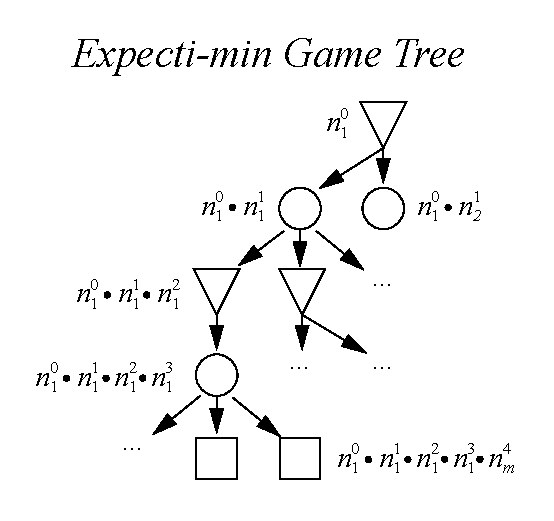
\includegraphics[width=0.49\textwidth,height=0.23\textheight,keepaspectratio]{figures/game-tree.pdf}
%  \hfill
% 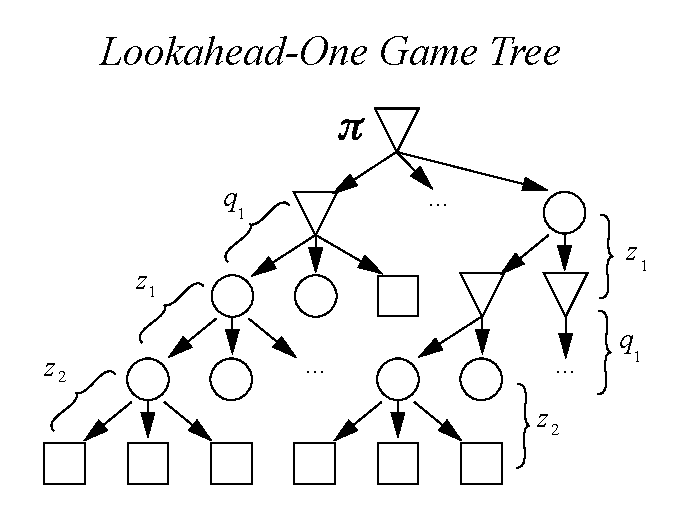
\includegraphics[width=0.49\textwidth,height=0.23\textheight,keepaspectratio]{figures/lookahead-one.pdf}
%  \caption{Monte Carlo tree search}
%\label{fig:mcts}
%\end{figure}
%
%\paragraph{Expectimin trees and optimal policies.}
%Let $\sT(\sN)$ be a expectimin tree with nodes $\sN$ (\figureref{mcts}).
%Each node $n \in \sN$ has a type $n.\sctype$ which is one of $\scmin$ (represented with inverted triangles), $\scexpect$ (represented with circles) or $\scvalue$ (represented with a square) and has children $n.\scchildren \subset \sN$.
%Additionally, nodes of type $\scvalue$ have a value $n.\scvalue$.
%The value of a node can be easily computed recursively: 
%\begin{align*}
%  \scvalue(n) &=
%  \begin{cases}
%    \min_{n'\in n.\scchildren} \scvalue(n') & \textrm{if}~n.\sctype = \scmin \\
%    \E_{n'\sim n.\scchildren}[\scvalue(n')] & \textrm{if}~n.\sctype = \scexpect \\
%    n.\scvalue & \textrm{if}~n.\sctype = \scvalue
%  \end{cases}.
%\end{align*}
%Additionally, an expectimin policy $\pi^*$ at a $\scmin$ node returns the child with the minimum value: $\pi^*(n) = \argmin_{n' \in n.\scchildren} \scvalue(n')$.
%As a concrete example, consider the expectimin tree in \figureref{mcts}. The value of the root node $n_1^0$ is,
%\begin{align*}
%  \scvalue(n_1^0) &= \min_{n_1^0.n_i^1} \E_{n_1^0.n_i^1.n_j^2} \left[\min_{n_1^0.n_i^1.n_j^2.n_k^3} \E_{n_1^0.n_i^1.n_j^2.n_k^3.n_l^4} \left[n_1^0.n_i^1.n_j^2.n_k^3.n_l^4.\scvalue \right] \right].
%\end{align*}
%
%\paragraph{Choosing queries $q_m$ with an expectimax tree.}
%Let us now formalize our decision problem as an expectimin tree, $\sT$.
%The nodes of the tree need to encapsulate as current state, the current time, $t$, the list of queries pending responses $Q = \{(q_1, t_1), \ldots, (q_m, t_m)\}$, where $q_i$ are the queries and $t_i$ is the time at which the query responds (we will compute an expectation over this quantity) and the received responses $Z = \{z_1, \ldots, z_l\}$.
%Without loss of generality, assume that $Q$ is sorted so that $t_1$ is closest in time to $t$.
%Let the root of $\sT$ be the $\min$ node $\scchoose(t, Q, Z)$, 
%with children $\scchoose(t, Q, Z).\turnin$, $\scchoose(t, Q, Z).\wait$ and $\scchoose(t, Q, Z).\query(q)$ for $q \in [n]$.
%$\scchoose(t, Q, Z).\turnin$ is a $\scvalue$ node with value equal to the expected loss of making a prediction in the current state:
%\[
%\scchoose(t, Q, Z).\turnin.\scvalue 
%= \E_{\by \sim \p(\cdot \given \bx, Z)}[\ell_{\rmclass}(\by, \byt)] + C(Q, t).
%\]
%$\scchoose(t, Q, Z).\wait$ is an $\scexpect$ node children $\{\scchoose(t', Q', Z') | t' = t_1, Q' = Q \setminus (q_1, t_1) Z' = Z \union {z_{l+1}} \forall z_{l+1} \in [L]\}$.
%Intuitively, choosing the $\wait$ node waits for the next response by advancing time and updating the query and response states.
%Finally,
%$\scchoose(t, Q, Z).\query(q)$ is an $\scexpect$ node that results in children 
%$\{\scchoose(t, Q', Z) | Q' = Q \union (q, t'), t' = t + \tau_q, \tau_q \sim \Gamma\}$: the $\query$ node places a new query and its expected time of response to $Q$. 
%
%\figureref{mcts} shows a simplified tree ignoring time constructed with a single query in flight; the root node is $\scchoose(\cdot, \{(q_1, t_1)\}, \{\})$. The branch on the left shows the expansion of the game tree along the child that chooses to query immediately, while the branch on the right considers the case where we wait to receive the first response ($z_1$) before querying ($q_2$).
%In the latter scenario, we may choose not to query again if the response we receive provides enough information.

%As described in \sectionref{model}, we would like to select and schedule several requests for labels to maximize our accuracy on predictions while trading off the cost and response time. 
%We view the problem in the Bayesian decision theoretic setting: what is the optimal behavioral policy under our current beliefs?
%The delay in the information we receive from label requests requires us to reason about time and the possible interactions between the responses we will receive.
%In this section, we describe how these interactions can be described using an expectimax tree.
%However, evaluating the optimal policy from the expectimax tree is intractable.
%We propose a Monte Carlo search based algorithm to efficiently approximate the optimal policy.


\section{Modeling human error}
\label{sec:human-error}

\pl{should we have this entire section up front;
it seems like you have to talk about human error in the original framework}

Accurately identifying and hence modeling labeling noise is important if we would like to maximize the information we can get from labelers.


\todo{(arun): rewrite}

Our learner will be allowed to query humans for additional certainty about individual random variables (nodes) $X_i$.
 Humans will exist in a pool $\sP$.
 An individual human $o_i \in \sP$ (for ``oracle'', using the loosest possible definition of oracle) has a model for expected behavior.
Our learner will be allowed to query humans for additional certainty about individual random variables (nodes) $X_i$.
 Humans will exist in a pool $\sP$.
 An individual human $o_i \in \sP$ (for ``oracle'', using the loosest possible definition of oracle) has a model for expected behavior. Specifically, we model the $o_i$ expected delay to respond to a question, and the error function (i.e. response given the true state of the world $h_{\text{true}}$).

For this work we use a simplified model of error, shared uniformly across crowd workers.
 Previous work \cite{yan2011active} \cite{donmez2008proactive} \cite{golovin2010near} has shown that in an offline setting treating oracles uniformly leads to a loss, but in practice our pool is churning so quickly that we don't have time to learn accurate distinctions between workers.
 We leave a solution to this problem to future work.

When asked about variable $X_j$, human error is modeled as correct (returns $h_{\text{true}}(X_j)$) with probability $1-\epsilon$, and chosen uniformly at random from $D_j$ with probability $\epsilon$.
 We use the notation $Q(o_i, X_j)$ to denote the response from asking human $i$ about random variable $j$.

\begin{equation}
    Q(o_i, X_j) \sim
    \begin{cases}
       \text{uniformly drawn from } D_j = \{1 \ldots K_j\}, & \text{with probability}\ \epsilon \\
      h_{\text{true}}(X_j), & \text{otherwise}
    \end{cases}
 \end{equation}
 
This answer arrives after a delay.
 We model the amount of time the worker takes to answer with a gaussian, parameterized by $\mu$ and $\sigma$.
 We use the notation $\sD(o_i, X_j)$ to denote the delay in response when asking human $i$ about random variable $j$.

\[\sD(o_i, X_j) \sim \sN(\mu, \sigma^2)\]

This is an imperfect model, since it assigns some mass to a negative response time, which is impossible, but given a large $\mu$ and relatively small $\sigma$ the mass assigned to $\sD(o_i, X_j) < 0$ is negligible, and it otherwise accurately reflects human response times.

%\section{Partial Monitoring Game}
\label{sec:partial}

To cast this problem as a Partial Monitoring Game, we must first make sure the outcome space $\sS$ is finite, which requires that we discretize time into epochs of length $t_{\text{epoch}}$, and impose a time limit on the game, $t_{\text{max}}$, resulting in a finite game space $\sS_{\text{discrete}}$.

\todo{details on how Partial Monitoring Games work}

We can define the entries of our loss matrix $L$ with respect to our loss function $\sL(h_{\text{final}}, h, m, t)$.
 The language $\Sigma$ used to populate our observability matrix $H$ is defined as the state space of the game $\sS_{\text{discrete}}$.

\todo{do math... borrow bounds from Bartok et. al, show Pareto optimal policy}

Our goal is to pick a policy $\pi^*$ to minimize the loss in the terminal state of the algorithm $s_{\text{final}}$.
 Since our loss term depends on the true state of the world $\theta^* = (h_{\text{true}}, t, m)$, of which only $t$ and $m$ are ever known, we can't do this directly.
 However, we have a distribution over our beliefs $p(h_{\text{true}})$ at every step (and consequently the state of the true state of the world $\theta^*$, since $t$ and $m$ are known), so we instead minimize \textit{risk}, which is defined with respect to a particular state of the world $\tilde{\theta}$ as
\[E_{\Theta \sim p(\theta)}[Loss(\Theta || \tilde{\theta})] = \int_{\theta} Loss(\theta || \tilde{\theta})p(\theta)d\theta\]

We can formulate our goal in concrete terms as follows:
\begin{equation*}
\begin{aligned}
& \underset{\pi}{\text{minimize}}
& & E_{\pi}[E_{h \sim p(h)}[\sL(h_{\text{final}}, h, m, t)]] \\
%& \text{subject to}
%& & a \in \sA
\end{aligned}
\end{equation*}

This reduces to the Optimal Decision Tree problem, which is NP-hard.


\section{Related Work}
\label{sec:related}

\todo{(arun): This section is currently a whole page long! We need to cut somewhere}

Our work brings together ideas from the active classification and learning literature as well as literature on collective intelligence systems from the human computer interaction community.
Our focus has been to address the practically relevant questions that arise at the watershed of these two fields: how to optimally classify instances in {\em real-time} allowing {\em queries} to {\em noisy oracles}. 
In this section, we review prior work and situate our own work within the literature.

\paragraph{Active learning and active classification}
In the traditional active learning setup, we are provided a large pool of unlabeled instances from which we must chose a subset to label. The goal is to pick a subset that minimizes the risk of the classifier obtained by training on that subset. 
Active learning has also been studied in the so-called streaming setting~\cite{agarwal2013selective,cheng2013feedback,chu2011unbiased,helmbold1997some,vzliobaite2011active} where the pool of examples is divided into smaller chunks; the most useful instances within each chunk are chosen to be labeled.
In either case, such a pool of examples is not available in our setting and we must make querying decisions sequentially on each input, i.e.\ at test time.
Our decision criteria is no longer which instance is optimal to label, but whether (partially) labeling an instance is worth the cost or not.

Active classification~\cite{greiner2002learning} also makes decisions at test time, but tries to find the {\em most informative feature} to measure.
One could view our measurements as high-informative features, however our work differs in two respects: we never get to actually observe the true labels and our system is evaluated on regret as opposed to classifier risk.
Greiner et al.~\cite{greiner2002learning} study the theoretical properties of active classification with the PAC framework.
Chai et al.~\cite{chai2004test} and Esmeir et al.~\cite{esmeir2007anytime} propose algorithms for active classification in the context of naive Bayes and decision trees respectively. Both algorithms rely on having a fully labeled dataset which is used to learn when certain features should be queried.

Despite the differences highlighted above, literature on active learning and active classification is very relevant because of the application of Bayesian decision theory to graphical models. 
Settles et al.~\cite{settles2008analysis} compare different utility choices when querying for complete labels for a CRF sequence model.
There is little existing work on querying a subset of the labels within a single structured output problem.
Angeli et al.~\cite{angeli2014combining} identify instances to label within a cluster of examples in a distantly supervised setting. While this choice was a subset of the labels in the graphical model, interactions between other labels in cluster were not considered.
Liang et al.~\cite{liang09measurements} introduced the measurement framework and studied the problem of active selection of measurements. However, the measurements considered were aggregated across the dataset (e.g.\ the expected proportion of a label), rather than label measurements within an instance.

\pl{well, within an example in some sense is a special case and the easy part, so you shouldn't use this as the contrast}

Finally, existing work~\cite{donmez2008proactive,golovin2010near,yan2011active,vijayanarasimhan2014large} has considered choosing measurements from multiple noisy oracles with heterogeneous costs.
We refer the reader to \cite{settles2010active} for a survey of active learning and its variants.


% This is more of a UI sort of thing, not really useful to us.
%~\cite{roth2006active} and~\cite{culotta2005reducing}, where humans perform top-K selection over model predictions.
%The systems fall back by stages to traditional no-assistance annotation if the top-K doesn't contain the any correct information.

% Ignoring Tong et. al because it's complex and doesn't quite handle this structured thing. It's about sampling for variables conditioned on somethin.
%jit in the context of fully Bayesian networks where the oracle can draw samples conditioned on certain ``controllable'' values - introduce the notion of expected posterior risk - something we also use.


% While this approach is effective when possible, it relies on the model to consistently produce the correct answer in a top-K for some very small $K$, so for large output spaces it breaks down.

%\paragraph{Noisy oracles}
%
%There's been a line of work on Active Learning in the context of multiple noisy, expensive oracles (\cite{donmez2008proactive,golovin2010near,yan2011active,vijayanarasimhan2014large}).
%This work tries to relax the traditional assumptions in active learning that the oracle is infallible and has no economic cost.
%Some of this work is directly motivated by applications to crowd-sourcing platforms that we investigate.
%WHY DIFFERENT?

% Bayesian priors we use not.
%Finally Bayesian active learning (\cite{golovin2010near},~\cite{tong2000active}) allows us to incorporate a Bayesian prior over our data, and we'll use this as a foundation for our approach to solving the asynchronous behavior problem.

\paragraph{Collective intelligence systems}

Using crowd workers to assist labeling tasks is an area of active research within the HCI community.
\textit{Flock}~\cite{chengflock} first crowdsources the identification of features for an image classification task, and then asks the crowd to annotate examples.
Our work seeks to make the second step more cost-effective by only querying the crowd when needed.
In another line of work, \textit{TurKontrol}~\cite{peng2010decision} models individual crowd worker reliability to optimize the number of human votes needed to achieve confident consensus using a POMDP.
We also model the reliability of workers though using an unsupervised model, similar to \findcite{crowd em}.
Finally, recent work has studied how to support real-time behavior with crowd workers~\cite{bernstein2011crowds,lasecki2013real} by hiring workers ``on retainer''.
We use the same retainer model to maintain a pool of real-time crowd workers with low response times.

% Using crowds to power decision making is not a new idea. Systems in this space that support real-time behavior include \textit{Adrenaline}~\cite{bernstein2011crowds} and \textit{Legion AR}~\cite{lasecki2013real}, which both use a system where crowds are recruited ``on-retainer'' in order to be available at a moments notice.
% We use the same retainer model to maintain a pool of real-time workers with low response times.
%Using artificial-intelligence-crowd hybrids for time-insensitive workflows has also been previously explored.
%It makes no effort to train a model to augment or take over from the workers, so costs remain constant over time.
%Empirical studies have shown that this is an effective method for managing complex workflows \cite{peng2011artificial}.
%Our work follows \cite{peng2010decision} in that we apply Decision Theory to the problem of when to query the crowd, but we train a model to take over for the workers over time, and we handle the additional real time response constraint.

\paragraph{Partial monitoring games}
\noteb{This bullet point is actually to motivate that our problem is theoretically feasible.}
Our evaluation metric is unique in the active learning space in that consider a loss we do not observe because we never receive true labels.
By treating the measurements as partial feedback, our work can be theoretically modeled as a partial monitoring game\cite{cesabianchi06regret} and, in particular, an instance of the label-efficient learning problem\cite{cesabianchi05minimizing}.
Cesa-Bianchi et al.~\cite{cesabianchi06regret} show that in the online setting, the regret of a partial monitoring game is lower bounded by $O(T^{2/3})$, where $T$ is the number of examples seen. They also provide an algorithm that meets this bound: use the current model to pick the best label and query for complete labels at random with a small probability to update your model.
These guarantees provide theoretical foundation for our work.

\section{Experiments}
\label{sec:experiments}

% === Figures
\begin{table}[t]
  \begin{tabular}{l p{0.4\textwidth} p{0.4\textwidth} r r r}
    {\bf Dataset (Examples)} & {\bf Task and notes} & {\bf Features} \\ \hline
  {\bf NER (1000)}     & 
    We evaluate on a simplified version of CoNLL-2003 NER task\tablefootnote{\href{http://www.cnts.ua.ac.be/conll2003/ner/}{http://www.cnts.ua.ac.be/conll2003/ner/}}, a sequence labeling problem over English sentences. 
    We only consider the three entity tags corresponding to persons ($\textsc{per}$), locations ($\textsc{loc}$) or others ($\textsc{o}$)\tablefootnote{%
    The original also includes the tags $\textsc{org}$ and $\textsc{misc}$, however the distinctions between these tags are artificial, making it very difficult for non-expert crowd workers to provide accurate labels.}.
    &
    We used standard features~\cite{finkel2005incorporating}: the current word, current lemma, previous and next lemmas, lemmas in a window of size three to the left and right, word shape and word prefix and suffixes. \\
  {\bf Sentiment (1800)} & 
    We evaluate on a subset of the Stanford sentiment dataset\cite{maas2011learning} that consists of 2000 polar movie reviews; the goal is binary classification of documents into classes $\textsc{pos}$ and $\textsc{neg}$. 
    &
    We used two feature sets, the first (\textsc{bigrams}) containing only word unigrams and bigrams, and the second (\textsc{rnn}) that also contained sentence vector embeddings from~\cite{socher2013recursive}.
    \\
  {\bf Face (1784)} & 
  We evaluate on a celebrity face classification task\tablefootnote{\todo{}}. Each image must be labeled as one of the following four choices: Andersen Cooper, Daniel Craig, Scarlet Johansson and Miley Cyrus.
    &
    We used the last layer of a 11-layer AlexNet~\cite{krizhevsky2012imagenet} trained on ImageNet as input feature embeddings.
\end{tabular}
  \caption{Datasets used in this paper and number of examples we evaluate on.}
\label{tbl:dataset}
\end{table}

\begin{table}[t]
%% NER 
\begin{tabular}{l r r r r r | r r r r r}
  \multicolumn{6}{c|}{Named Entity Recognition} & 
      \multicolumn{3}{c}{Face Identification} \\
      \textbf{System} & \textbf{Latency} & \textbf{Qus./tok} & \textbf{P} & \textbf{R} & \textbf{F$_1$} 
          & \textbf{Latency} & \textbf{Qus./ex} & \textbf{Acc.} 
    \\ \hline
    1-vote & 664 ms & 1.0 & 66.38 & 89.58 & 76.15 
      & %1-vote & 
      1414 ms & 1.0 & 87.75 \\ %\hline
    3-vote & 1495 ms & 3.0 & 92.79 & 89.56 & 91.58 
        & %3-vote &
        1865 ms & 3.0 & 88.44 \\ %\hline
    5-vote & 3887 ms & 5.0 & 98.25 & 92.33 & 95.20 
        & 
        & -- & -- & -- \\
    Offline & n/a & n/a & 62.38 & 69.76 & 65.86 
        % Offline 
        & n/a & n/a & 87.43 \\    %\hline
    Entropic & 1523 ms & 0.65 & 91.74 & 90.90 & 91.33 
        % Entropic 
        & 1121 ms & 1.12 & \textbf{91.53} \\ %\hline
    \textbf{LENSE} & 3368 ms & \textbf{0.62} & \textbf{94.32} & \textbf{93.16} & \textbf{93.73} 
    %\textbf{LENSE} 
    & 961 ms & \textbf{1.06} & 88.45 \\   %\hline
\end{tabular}
\caption{Results on NER and Sentiment tasks comparing latencies, queries per token and performance metrics (Precision, Recall and \fone{} for NER and accuracy for Sentiment).}
\label{tbl:results}
\end{table}

\begin{table}[t]
    \begin{minipage}[t]{.49\textwidth }
        \begin{tabular}[b]{l  r  r  r  r}
    %\hline
    \textbf{System} & \textbf{Latency} & \textbf{Qu./ex} & \textbf{Acc.} \\ \hline
    1-vote & 6.6 s & 1.00 & 89.2 \\ %\hline
    3-vote & 10.9 s & 3.00 & 95.8 \\ %\hline
    5-vote & 13.5 s & 5.00 & 98.7 \\ %\hline
    \multicolumn{5}{c}{\textsc{bigrams}} \\ \hline
%Bigrams: \\
    Offline & n/a & n/a & TODO \\ %\hline
    \textbf{Threshold} & TODO s & TODO & TODO \\ %\hline
    LENSE & 18.1 s & 3.48 & 98.6 \\ %\hline
    \multicolumn{5}{c}{\textsc{rnn}} \\ \hline
    Offline & n/a & n/a & TODO \\ %\hline
    \textbf{Threshold} & 11.0 s & 2.85 & 96.0 \\ %\hline
    \textbf{LENSE} & 16.1 s & 3.19 & 98.6 \\% \hline
\end{tabular}

        \caption{Results on the Sentiment task comparing latency, queries per example and accuracy.}
        \label{tbl:sentiment-results}
        \vfill
    \end{minipage}%
    \begin{minipage}[t]{.49\textwidth}
  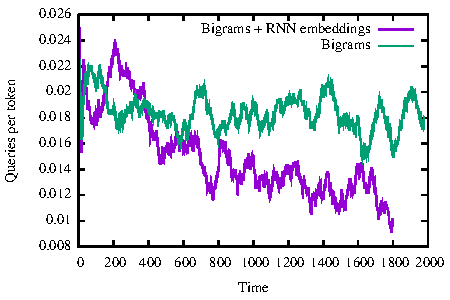
\includegraphics[width=\textwidth]{figures/sentiment_cost_per_token_vs_time/cost_per_token_vs_time.pdf}
  \captionof{figure}{Queries per example over time for the LENSE on Sentiment. With simple \textsc{bigram} features, the model does not have the capacity to predict at our desired accuracy and must query the crowd. With more complex \textsc{rnn} features, the model learns and queries the crowd less over time.}
        \label{fig:sentiment-tradeoff}
    \end{minipage}
\end{table}

% === Other stuff.

In this section, we empirically evaluate our approach on three tasks. 
While on-the-job setting we propose is targeted at scenarios where there is no data to begin with, we use existing labeled datasets (\tableref{dataset}) to empirically evaluate the performance of our system relative to baselines.

\paragraph{Baselines.}
We evaluated the following four methods on each dataset:
\begin{enumerate}
  \item {\bf Human n-query}: The majority vote of $n$ human crowd workers was used as a prediction.
  \item {\bf Offline baseline}:
    Uses a classifier that trains on the gold output for all examples seen so far and then returns the MLE as a prediction.
    This is the best possible offline system: it sees perfect information about all the data seen so far, but can not query the crowd while making a prediction.
  \item {\bf Entropic threshold}: Uses a heuristic on-the-job learning agent to make predictions. 
    The agent queries any labels that it estimates to have a marginal probability below a threshold $k = 0.88$. % \footnote{We found $k = 0.88$ to give the best results on our datasets.}
    Instead of computing the expected marginals over the responses to queries in flight, the agent simply reduces the uncertainty by a factor of $0.3$ and makes multiple requests until the threshold is crossed. Predictions are made using MLE on the model given responses.
    The agent does not reason about time and makes all its queries at the very beginning.
  \item {\bf LENSE:} Our full system as described in \sectionref{async}.
\end{enumerate}

To initialize parameters for the model-based methods, we used a burn-in period of 40 examples which were used to get labels on everything. We used those responses to train initial parameters for the prediction model $\theta$, response model $\beta$ and delay model $\Gamma$.
We do not update parameters for the delay and response models online.

\paragraph{Implementation and crowdsourcing setup.}
We implemented the retainer model of~\cite{bernstein2011crowds} on Amazon Mechanical Turk to create a ``pool'' of crowd workers that could respond to queries in real-time.
The workers were given a short tutorial on each task before joining the pool to minimize systematic errors caused by misunderstanding the task.
We paid Workers \$1.0 to join the retainer pool and an additional \$0.01 per query.
Worker response times were generally in the range of 3-6 seconds for NER, 10-15 seconds for Sentiment, and 2-4 seconds for Faces.

When running experiments, we found that the results varied based on the current worker quality. %, fluctuating on the NER task between 87 and 96 F1, depending on workers.
To control for variance in worker quality across our evaluations of the different methods, we collected 5 worker responses and their delays on each label ahead of time\footnote{If accepted, we will make our datasets of frozen human responses, delays, and anonymized worker tags publicly available}.
During simulation we sample the worker responses and delays without replacement from this frozen pool of worker responses. 
Neither LENSE nor the entropic threshold needed more than 3 queries on a single label.

% DETAILS
% Anecdotally, we also report a range of results on 5 complete runs of our system using {\em real live crowd workers}, recruited at test time, over the first 150 sentences of our dataset. The results exhibit high variance based on worker quality.
%
%\begin{center}
%\begin{tabular}{ | r | r | r | r | r | }
%    \hline
%    Time/token & Requests/token & Precision & Recall & F1 \\ \hline
%    1444 ms - 3426 ms & 0.54 - 0.66 & 92.9 - 96.91 & 82.50 - 94.01 & 87.4 - 95.43 \\ \hline
%\end{tabular}
%\end{center}
%
%Filtering workers while running, or inferring separate error models for each worker, would clearly deliver substantial gains in reliability over a system that assumes uniform quality. We leave this to future work.

\paragraph{Summary of results.}
\tableref{results} summarizes the performance of the methods on the three tasks.
On all three datasets, we found that on-the-job learning outperforms machine and human-only comparisons on both quality and cost. 
On NER, we achieve an \fone{} of $93.7\%$ at roughly 1/6th the cost of achieving the same result using the human-only approach. On Sentiment and Faces, we reduce costs for a comparable accuracy by a factor of 3-4.
For the latter two tasks, both on-the-job learning methods, entropic threshold baseline and LENSE, perform comparably.
The simple heuristic adopted by the entropic threshold baseline is sufficient to reason about expected marginals on both these tasks because they are single label prediction tasks which do not involve any interactions between labels.

\begin{figure}[t]
  \centering
  \begin{subfigure}[b]{0.49\textwidth}
  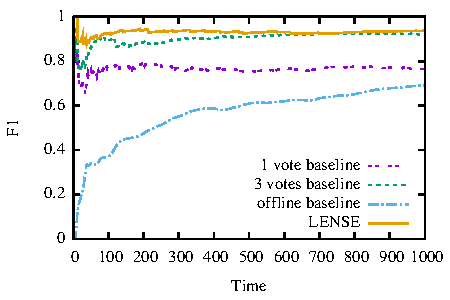
\includegraphics[width=\textwidth]{figures/ner_2_class/f1_plot/f1_vs_time.pdf}
\end{subfigure}
  \begin{subfigure}[b]{0.49\textwidth}
  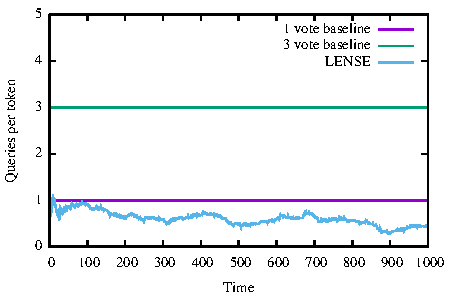
\includegraphics[width=\textwidth]{figures/ner_2_class/cost_plot/cost_vs_time.pdf}
  \end{subfigure}
  \caption{Comparing \fone{} and queries per token on the NER task. LENSE maintains high \fone{} scores by querying the crowd when it is unsure. As the model learns, it needs to query the crowd less.}
\label{fig:ner-f1}
\end{figure}

%\paragraph{Does the model respect accuracy preferences?} 
\figureref{ner-f1} tracks the performance and cost of LENSE over time on the NER task.
LENSE is not only able  to consistently outperform other baselines, but the cost of the system steadily reduces over time.
On the NER task, we find that LENSE is able to trade off time to produce more accurate results than the entropic threshold baseline with fewer queries by waiting for responses before making another query.

% == DEV F1
%We also plot \fone{} on a held-out set: while we receive noisy and sparse supervision LENSE is able to train a classifier that generalizes well over time. 
%Compared to the offline baseline, which sees perfect labels on all examples, LENSE observed labels on only \ac{KEENON: fix this number: 600} words. For a comparable number of tokens, the offline baseline has an \fone of \ac{KEENON: fix: 63\%}.

% === Compare with entropic threshold
%\paragraph{Why is the Entropic threshold system so much better on sentiment and faces?}
%LENSE exploits structure in the model when querying, and so outperforms the Entropic threshold in the presence of structure (see NER task results).
%However, when neither structure or time pressure is present, LENSE's only signal is the entropy of the prediction, and so the Entropic threshold is able to perform just as well, if not slightly better when the threshold is optimally set.

%We note that although our model is receiving supervisition signal at roughly 1/15 the rate of a fully observed online learning scenario\footnote{this calculation assumes ``fully observed'' is approximated by 3 human labels per example}, we track roughly parallel to the fully supervised line.

%\paragraph{In the limit, would LENSE still need crowd supervision?}
While on-the-job training allows us to deploy quickly and ensure good results, we would like to eventually operate without crowd supervision.
%In order to do so, we must ensure that our model has the capacity to keep learning from the crowd.
\figureref{sentiment-tradeoff}, we show the number of queries per example on Sentiment with two different features sets, \textsc{bigrams} and \textsc{rnn} (as described in \tableref{datasets}).
With simpler features (\textsc{bigrams}),
the model saturates early and we will continue to need to query to the crowd to achieve our accuracy target (as specified by the loss function).
On the other hand, using richer features (\textsc{rnn}) the model is able to learn from the crowd and the amount of supervision needed reduces over time.
%This suggests that given a sufficiently rich model, costs can be brought to zero in the limit.
Note that even when the model capacity is limited, LENSE is able to guarantee a consistent, high level of performance.

% -- CUT
%\paragraph{When does LENSE query?}
%During the initial stages of learning for the NER task, LENSE made multiple queries on all tokens.
%After a few examples, though, LENSE focused its queries on unseen entity tokens.
%Consider the following example taken from our run logs: \textit{``U.S.\ says still committed to Cuba migration pacts''}.
%%For example, after seeing \ac{600} examples, 
%The model has already seen {\it U.S.\/} and predicts that it is a \scloc{} with 97\% probability.
%On the other hand, having never seen the token {\it Cuba\/} before, the model starts with a belief that {\it Cuba\/} is 59\% \scper, 37\% \scloc{} and 3\% \scnone.
%It immediately fires off two queries about {\it Cuba\/} and waits 4 seconds for both responses to return \scloc{}.
%The model now believes that {\it Cuba\/} is \scloc{} with 95\% probability and returns its prediction.
%This demonstrates that using the model allows LENSE to focus supervision to where it is needed.


% \paragraph{Are we learning a good model?}
% We receive very noisy and sparse supervision.
% Despite this, to reduce the costs in the future, our system must learn to generalize well.
% We refer to \figureref{ner-dev-f1}.
% We note that although our model is receiving supervisition signal at roughly 1/15 the rate of a fully observed online learning scenario\footnote{this calculation assumes ``fully observed'' is approximated by 3 human labels per example}, we track roughly parallel to the fully supervised line.

% Held out figure for space concerns.
%\begin{figure}[t]
%  \begin{centering}
%  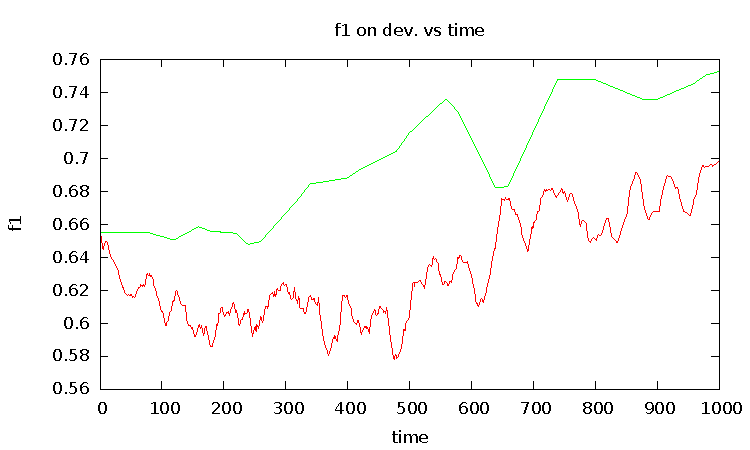
\includegraphics[width=1.0\textwidth]{figures/ner_2_class/machine_f1_plot/machine_f1_vs_time.pdf}
%  \end{centering}
%  \caption{A figure showing the relationship between the classifier we train, and one trained on gold labeled data. Evaluation is on a held out dev set. Note that our classifier learns more slowly because we are handing it a noisy approximation to train on, but the classifier narrows the gap as it gets more data.}
%\label{fig:ner-dev-f1}
%\end{figure}


\section{Conclusion}
\label{sec:conclusion}

We demonstrate a practical system to navigate the cost-delay-accuracy tradeoff surface by \textit{asynchronous active classification}.
 This system highlights the potential value of making the crowd available to machine-learning classifiers at test time, and we hope inspires further research in this promising direction.

Much of the research effort associated with demonstrating this system was ``plumbing,'' writing and debugging large pieces of logistical code for marshaling and managing the humans and machine learning algorithms in an asynchronous fashion.
% We have published an easily extensible and customizable base for further work in asynchronous active classification, which we call L.E.N.S.E. (Learning from Expensive, Noisy, Slow Experts) at \url{github.com/lense-project/lense-base}, that we hope proves useful.

\section{Future Work}

\begin{itemize}
  \item Arbitrary measurements.
\end{itemize}



% I don't think we need this just yet.
%\subsubsection*{Acknowledgments}
%
% Kelvin, Volodymyr for useful discussions.
% Amy for vision experiments.
% Anonymous reviewers for their helpful feedback.

\subsubsection*{References}

\bibliographystyle{plain}
\bibliography{ref,all}

\end{document}
